%%% The ``\documentclass'' command has one parameter, based on the kind of
%%% document you are preparing.
%%%
%%% [annual] - Technical paper accepted for presentation at the ACM SIGGRAPH 
%%%   or SIGGRAPH Asia annual conference.
%%% [sponsored] - Short or full-length technical paper accepted for 
%%%   presentation at an event sponsored by ACM SIGGRAPH
%%%   (but not the annual conference Technical Papers program).
%%% [abstract] - A one-page abstract of your accepted content
%%%   (Technical Sketches, Posters, Emerging Technologies, etc.). 
%%%   Content greater than one page in length should use the "[sponsored]"
%%%   parameter.
%%% [preprint] - A preprint version of your final content.
%%% [review] - A technical paper submitted for review. Includes line
%%%   numbers and anonymization of author and affiliation information.

\documentclass[abstract]{acmsiggraph}
\usepackage{verbatim} 
\usepackage{soul}
\usepackage{graphicx}


% Alter some LaTeX defaults for better treatment of figures:
    % See p.105 of "TeX Unbound" for suggested values.
    % See pp. 199-200 of Lamport's "LaTeX" book for details.
    %   General parameters, for ALL pages:
    \renewcommand{\topfraction}{0.9}	% max fraction of floats at top
    \renewcommand{\bottomfraction}{0.8}	% max fraction of floats at bottom
    \renewcommand{\dbltopfraction}{0.9}	% fit big float above 2-col. text
    \renewcommand{\textfraction}{0.07}	% allow minimal text w. figs
    %   Parameters for FLOAT pages (not text pages):
    \renewcommand{\floatpagefraction}{0.7}	% require fuller float pages
	% N.B.: floatpagefraction MUST be less than topfraction !!
    \renewcommand{\dblfloatpagefraction}{0.7}	% require fuller float pages

	

%%% If you are submitting your paper to one of our annual conferences - the 
%%% ACM SIGGRAPH conference held in North America, or the SIGGRAPH Asia 
%%% conference held in Southeast Asia - there are several commands you should 
%%% consider using in the preparation of your document.

%%% 1. ``\TOGonlineID''
%%% When you submit your paper for review, please use the ``\TOGonlineID''
%%% command to include the online ID value assigned to your paper by the
%%% submission management system. Replace '45678' with the value you were
%%% assigned.

\TOGonlineid{45678}

%%% 2. ``\TOGvolume'' and ``\TOGnumber''
%%% If you are preparing a preprint of your accepted paper, and your paper
%%% will be published in an issue of the ACM ``Transactions on Graphics''
%%% journal, replace the ``0'' values in the commands below with the correct
%%% volume and number values for that issue - you'll get them before your
%%% final paper is due.

\TOGvolume{0}
\TOGnumber{0}

%%% 3. ``TOGarticleDOI''
%%% The ``TOGarticleDOI'' command accepts the DOI information provided to you
%%% during production, and which makes up the URLs which identifies the ACM
%%% article page and direct PDF link in the ACM Digital Library.
%%% Replace ``1111111.2222222'' with the values you are given.

\TOGarticleDOI{1111111.2222222}

%%% 4. ``\TOGprojectURL'', ``\TOGvideoURL'', ``\TOGdataURL'', ``\TOGcodeURL''
%%% If you would like to include links to personal repositories for auxiliary
%%% material related your research contribution, you may use one or more of
%%% these commands to define an appropriate URL. The ``\TOGlinkslist'' command
%%% found just before the first section of your document will add hyperlinked
%%% icons to your document, in addition to hyperlinked icons which point to
%%% the ACM Digital Library article page and the ACM Digital Library-held PDF.

\TOGprojectURL{}
\TOGvideoURL{}
\TOGdataURL{}
\TOGcodeURL{}

%%% Replace ``PAPER TEMPLATE TITLE'' with the title of your paper or abstract.

%\title{Evaluation of a Tangible Interface for Architectural Daylighting}
\title{Evaluation of a Tangible Interface for Architectural Daylighting Analysis}

%%% The ``\author{}'' command takes the names and affiliations of each of the
%%% authors of your paper or abstract. The ``\thanks{}'' command takes the
%%% contact information for each author.
%%% For multiple authors, separate each author's information by the ``\and''
%%% command.

\author{Joshua D. Nasman\thanks{e-mail: nasmaj@cs.rpi.edu}\\ Rensselaer Polytechnic Institute %
\and Barbara Cutler\thanks{e-mail: cutler@cs.rpi.edu}\\ Rensselaer Polytechnic Institute }

%%% The ``pdfauthor'' command accepts the authors of the work,
%%% comma-delimited, and adds this information to the PDF metadata.

\pdfauthor{Joshua D. Nasman, Barbara Cutler}

%%% Keywords that describe your work. The ``\keywordlist'' command will print
%%% them out.

\keywords{augmented reality, daylighting design, user studies. \vspace{-0.05in}}

%%% The ``\begin{document}'' command is the start of the document.

%%% If you have user-defined macros, you may include them here.

% example of a user-defined macro called ``remark.''
% \newcommand{\remark}[1]{\textcolor{red}{#1}}

\begin{document}

%%% A ``teaser'' image appears under the title and affiliation information,
%%% horizontally centered, and above the two columns of text. This is OPTIONAL.
%%% If you choose to have a ``teaser'' image, it needs to be placed between
%%% ``\begin{document}'' and ``\maketitle.''

%\teaser{
%   \includegraphics[height=1.5in]{images/sampleteaser}
%   \caption{Spring Training 2009, Peoria, AZ.}
%}

%%% The ``\maketitle'' command must appear after ``\begin{document}'' and,
%%% if you have one, after the definition of your ``teaser'' image, and
%%% before the first ``\section'' command.

\maketitle

%%% Your paper's abstract goes in its own section.

\begin{abstract}

We present a study of a tangible user interface (TUI) for
architectural design and daylighting analysis.  This tool provides an
intuitive way for architects and future building occupants to quickly
construct physical models and then view a simulation of daylighting in
the model at interactive rates.
%
%\fbo{blah sentence}
%User studies are an effective way to obtain both qualitative and
%quantitative feedback for user interfaces.
%
We conducted
%investigate the results of 
a user study 
%of 13 participants 
of both formally-trained architects and non-architects in a set of analysis and design exercises.
%design and
%daylight analysis exercise.  
This study investigates the effectiveness of this interface as an
educational tool, the precision and accuracy of the constructed
physical models,
%how accurately users can model with the tool, and
and the overall effectiveness of the tangible interface.  The four
part study investigates users' intuitions about daylighting and their
interaction with the tool for analysis
%evaluating 
of an existing space, for proposing renovations to the space, and for
designing a totally new space with the same architectural program that
better addresses the occupants' needs.
%for the same to meet peoples' daylighting needs.  
%While completing these exercises 
These exercises revealed misconceptions in many of the participants'
intuitions about daylighting and overall the participants
%many users were surprised by
%unexpected simulation results and 
expressed interest in this simulation tool 
for daylighting analysis in architectural design.
%method for simulating daylighting within
%the space.



%\end{abstract}

%%% ACM Computing Review (CR) categories.
%%% See <http://www.acm.org/class/1998/> for details.
%%% The ``\CRcat'' command takes four arguments.

%\begin{CRcatlist}
%  \CRcat{I.3.7}{Computer Graphics}{Three-Dimensional Graphics and Realism}{Virtual Reality};
%\end{CRcatlist}

%%% The ``\keywordlist'' command prints out the keywords.

%\keywordlist

%%% The ``\TOGlinkslist'' command will insert hyperlinked icon(s) to your
%%% paper. This includes, at a minimum, hyperlinked icons to the ACM article
%%% page and the ACM Digital Library-held PDF. If you added URLs to
%%% ``\TOGprojectURL'' or the other, similar commands, they will be added to
%%% the list of icons.
%%% Note: this functionality only works for annual-conference papers.

%\TOGlinkslist

%%% The ``\copyrightspace'' command 
%%% Do not remove this command.

\copyrightspace

%%% This is the first section of the body of your paper.



Architectural daylighting design is the use of windows and reflective
surfaces to make effective use of natural light from the sun and sky
within a physical environment.  Increased use of daylighting can
reduce the need for supplemental electric lighting during the day,
decreasing operating costs and reducing the consumption of
non-renewable resources. 
%Furthermore, the dynamic time-varying and
%easonally-varying qualities of daylighting can make spaces with
%natural light more interesting and comfortable.  However, the
%distribution of daylighting within a building for a particular moment
%can be difficult for non-experts to accurately and quantitatively
%predict, and detailed simulations are expensive.  In a common design
%scenario for an office space, the typical goals for daylighting are to
%maximize the {\em daylight autonomy}, the number of hours per day/year
%that the work surfaces receive adequate lighting for reading.  Yet too
%much sunlight is also problematic: we must avoid the possibility of
%{\em glare}, reduced visibility for occupants of the space due to high
%contrast in light intensity within the visual field.\
\nocite{ShengYYC09} 
%
%In this paper we evaluate this Spatially Augmented Reality (SAR)
%system; a concept first introduced by {\em Shader Lamps} to project information
%onto existing surfaces in the real world~\
\nocite{Raskar:2001:SLA}

The daylighting analysis system simulates the complex inter-reflection
of natural light within a scene and uses a set of six standard office
projectors surrounding the table to ``paint'' the physical primitives
with the simulation results.  Designing in the tabletop system is done
by sketching with physical \emph{wall primitives} to create a closed
space with \emph{window primitives} that are placed over the top edge
of the walls.  A calibrated overhead camera captures the arrangement
of these elements and the geometry is converted into a closed triangle
mesh.  Radiosity, a patch-based lighting method, is used to simulate
light propagation within the space and the rendering system displays
the simulated natural lighting on the physical model using six
projectors positioned in a circle above the table.


% 
%
%We envision our tool being useful for a wide audience.  Not only will
%it be useful for architecture students and professional architects,
%but also for interior designer and future occupants working on 
%tasks
%such as furniture placement.
%
%Our initial user study of this interface had
%thirteen student participants: six architecture majors and seven
%non-architects (five of which have some general design training).
%

The contributions of our work:

\begin{itemize}

\item Exploration of participants' fundamental understanding of
  daylighting design, overlighting, underlighting and glare.\vspace{-0.03in}

\item Quantitative analysis of the users' accuracy in using our
  physical sketching system to model a room they had just visited.\vspace{-0.03in}

\item Evaluation of the participants' use of our tool and their
  perception of quantitative and qualitative daylighting from the
  displayed simulations.\vspace{-0.03in}

\item Demonstration of our tangible interface as a
  creativity-enhancing tool for architectural daylighting design.

\end{itemize}

\begin{figure}[t]
  \centering
  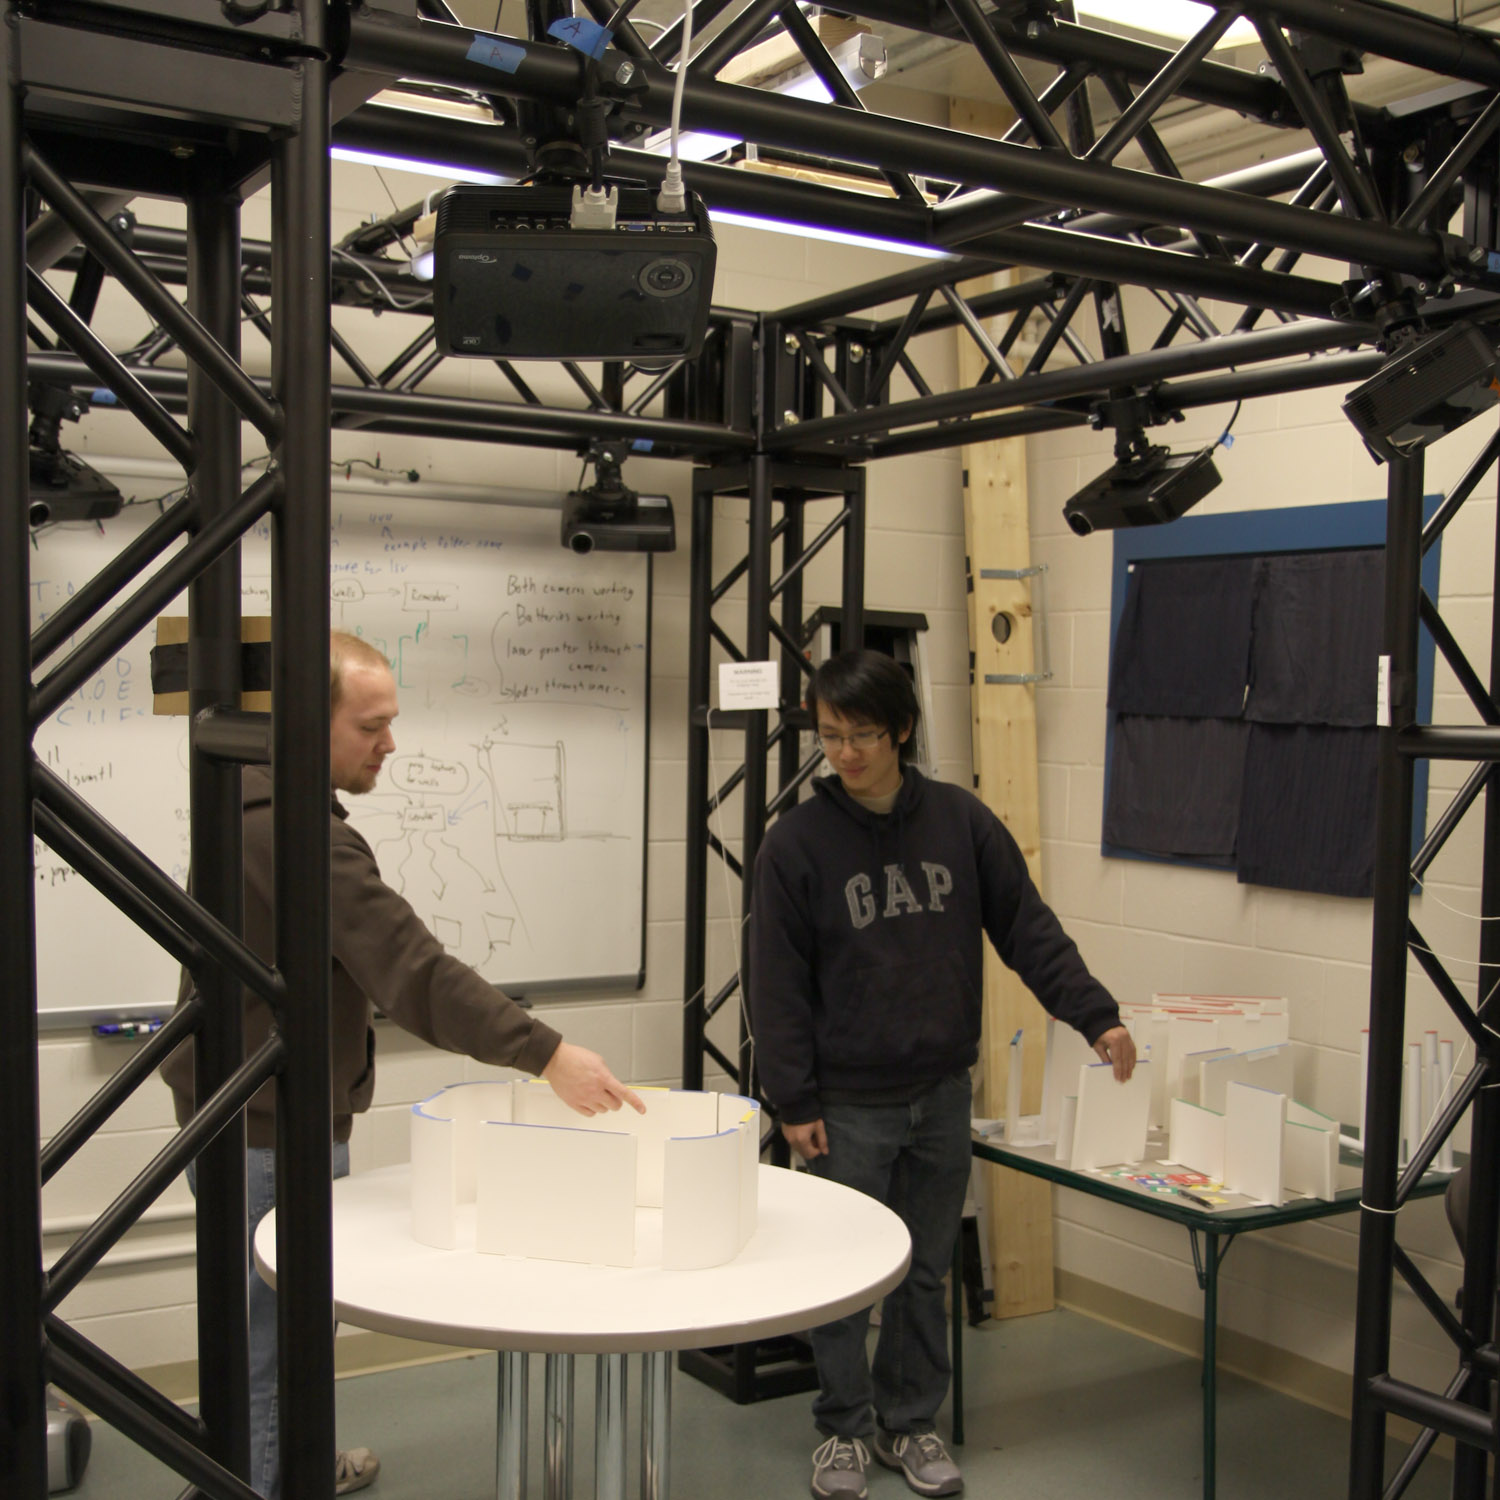
\includegraphics[width=1.65in]{images/photos/josh_jonathan_new_contraption}
  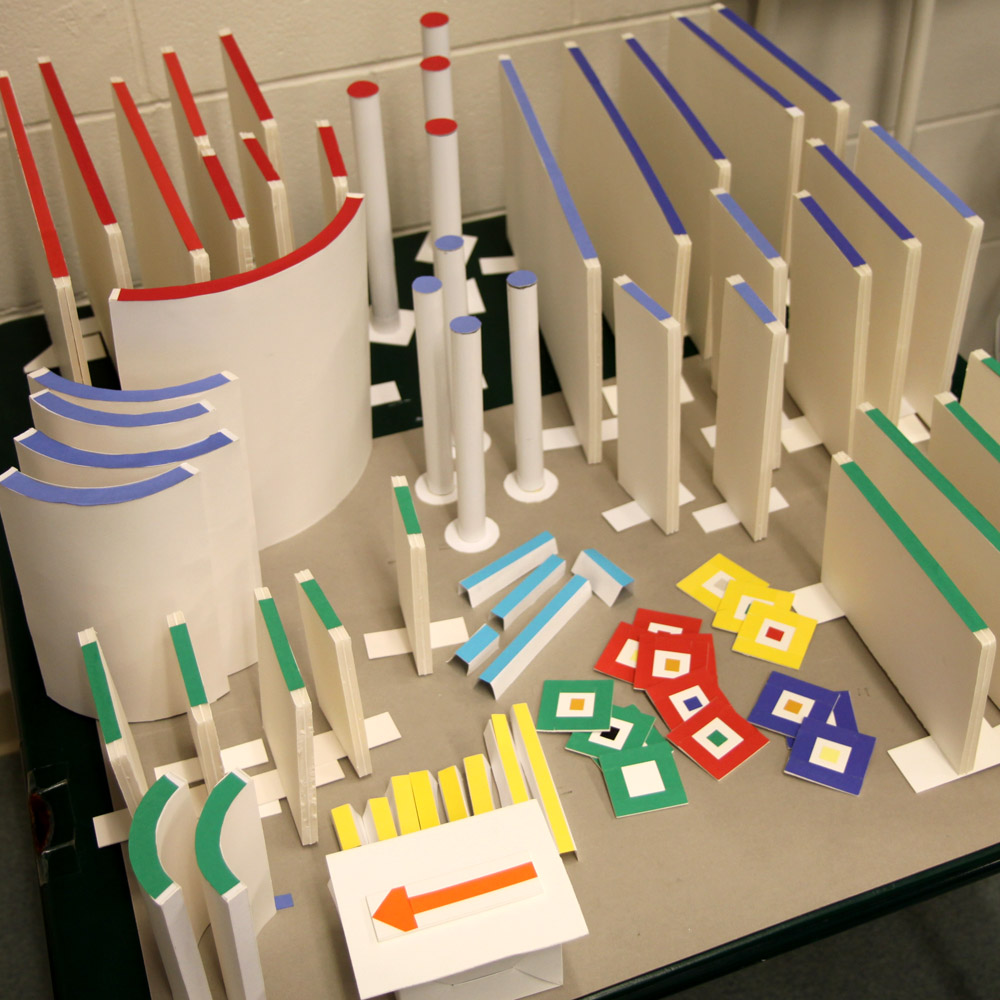
\includegraphics[width=1.65in]{images/photos/available_wall_pieces}\vspace{-0.19in}\\
\begin{minipage}{1.65in}~{\color{white}{\bf a)}}\end{minipage}
\begin{minipage}{1.65in}~{\color{white}{\bf b)}}\end{minipage}\vspace{0.05in}\\
  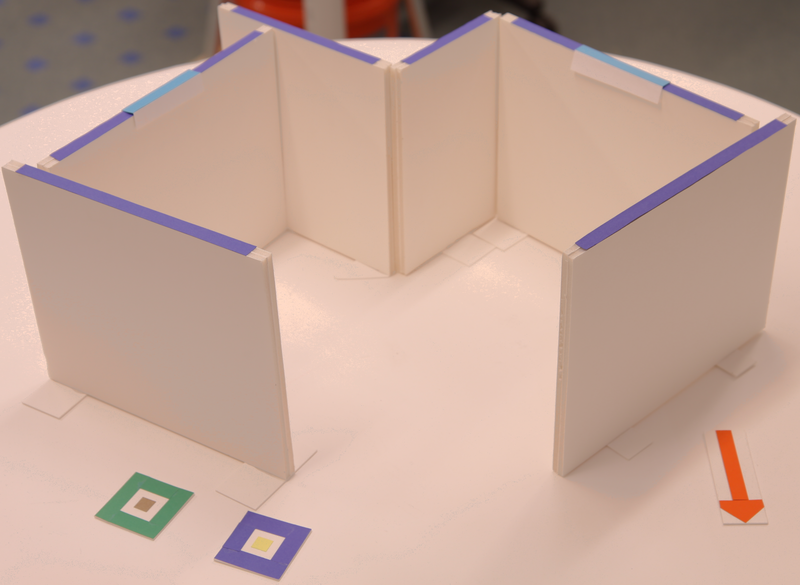
\includegraphics[width=1.65in]{images/photos/sample_model}
  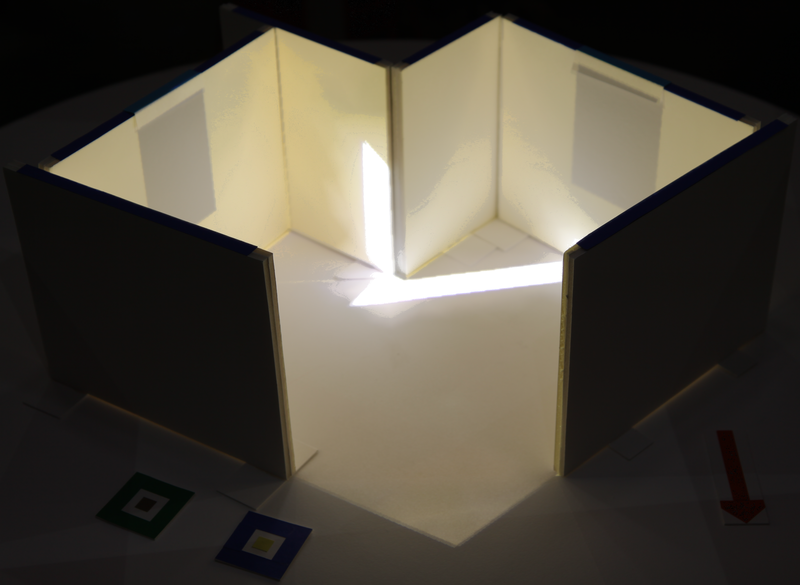
\includegraphics[width=1.65in]{images/photos/sample_rendering}\vspace{-0.19in}\\
\begin{minipage}{1.65in}~{\color{black}{\bf c)}}\end{minipage}
\begin{minipage}{1.65in}~{\color{white}{\bf d)}}\end{minipage}\vspace{-0.00in}\\
  \caption{Our new tangible user interface for architectural daylighting design allows
    multiple users to a) gather around a physical sketching
    environment and select from b) a set of wall primitives and window
    and material markers to c) build a rough sketch of an
    architectural design.  A d) visualization of a daylighting
    simulation is projected onto these surfaces. }
\vspace{-0.1in}
  \label{figure:tabletop}
\end{figure}


Our study was divided into four consecutive tasks.  The first task was
designed to prime the user for thinking about daylighting and gauge
the user's pre-existing intuition about daylighting.  
%The other three
%tasks had the participant work with the TUI daylighting simulation
%system.  Thus, prior to the second task, a brief, 5-minute
%introduction to the system was provided, including the modeling
%primitives available and how to request daylighting simulations of a
%specific time and day or a time-lapse animation of a complete day.
%
%The second, third, and forth tasks of the study were designed in the
%spirit of a \emph{cognitive walkthrough}, but with some guidance on
%tool use available during the study and a self-reflective
%pen-and-paper questionnaire completed by the user after each task.  In
%a cognitive walkthrough study the participant is given a task and the
%researchers observe the user as he/she performs the task.
%Because the system does have a set of primitives which must be
%understood, 
%Users were allowed to experiment with the TUI for daylighting
%simulation as they saw fit in completing the tasks.
%
For the second task, users were introduced to the TUI for daylighting
simulation and asked to construct and analyze a physical model of the
computer lab they had just visited. 
% and sketched in the previous
%section.
Then users were asked to propose and evaluate a modest renovation to
the existing space to improve the use of daylighting in the
space.  And finally, the users were encouraged to create a brand new
design and use the TUI to evaluate the resulting illumination.

%  Participants were then asked to use
%the simulation visualizations to evaluate the daylighting, requesting
%one or more static time or timelapse animations of particular days of
%the year.  The aim was to allow users to evaluate the accuracy of
%their predictions in Part 1.  Furthermore, by examining their choice
%of times and days selected, we can quantify the thoroughness of their
%exploration, and their understanding of the summer and winter solstice
%and the fall and spring equinox, and sunrise and sunset.

%Each of these tasks began with brief explanation (1-2 minutes), open
%exploration time with the tool in which participants created one or more
%models and viewed multiple daylighting simulations (5-20 minutes), and
%culminated with a questionnaire (10 minutes).  Users were encouraged
%to ask questions or provide feedback about the tool at any time.  The
%tasks were designed such that the study took approximately 1 to 2
%hours in total.


Participants in this study were significantly and positively
influenced by our tangible interface for daylighting simulation.
Users consistently claimed that their lighting intuition was improved, their design was aided by the tool, and that the interface was
accessible.  Many participants used the tool to look at lighting in
various seasons to understand how daylighting will vary throughout the
year.  Despite this, it was clear that users need additional
quantitative feedback and visualization
to more fully analyze glare in high contrast lighting conditions. 


%\vspace{-0.05in}
%\section{Related Work}
%\vspace{-0.05in}


%\fbox{ Tangible User Interfaces (TUIs) }

%Three prevalent themes in the field of Tangible User Interfaces (TUIs)
%are education, accuracy, and design.  
%The novel interactions made available by TUIs make them exciting
%candidates for alternate teaching techniques.  Furthermore, since TUIs
%feature list includes
%point and click interactions, layout design, and simulation, the
%accuracy of both the user's input and the user's perception of the
%output must be evaluated.  Since architecture is a design process of a
%tangible structure, many TUIs have focused on design tasks.


%\vspace{-0.05in}
%\subsection{Education and Information Tools}
%\vspace{-0.05in}

%TUIs inspire innovation in teaching and learning 
%through the opportunity to physically interact with data.
%
%Ishii and Ullmer present an interface of {\em phicons} (physical
%icons) and multiple display surfaces to navigate campus information.
%They combine a backprojected display and an LCD screen to create the
%{\em activeLENS}, which allows users to view an overview map and 3D
%information~\cite{Ishii97tangiblebits:}.
%
%Yee created a hybrid of this interface with a traditional interface
%for a workspace with a large passive 
%display and a smaller handheld display for 
%stylus input~\cite{642613}.  Unlike the activeLens, this system
%effectively utilizes both hands for data manipulation: one to hold and
%guide the lens and one for stylus input.  Maekawa
%extended the 
%ActiveLens-style display to
%a the surface of re-configurable blocks.  This display system maps the
%current 3D configuration to a database of shapes
%and displays on a small mobile screen the appropriate ``window'' into
%the corresponding virtual object~\cite{1517704}.  Jacob et
%al. developed the first system to directly project onto movable,
%tangible {\em pucks} for data manipulation~\cite{Jacob01atangible}.
%Spindler developed PaperLens~\cite{Spindler:2009:PAM:1731903.1731920},
%an interface using a tangible 2D display to show 3D information.
%Similarly, Song presents a tangible interface with a touch screen for
%displaying
%select planes of data based on its orientation relative to a large 2D
%display~\cite{Song:2011:WEA:1978942.1979140}.
%
%As illustrated by these TUIs and others, displays allowing physical
%5manipulation provide unique opportunities to visualize, organize,
%and understand data.

%\vspace{-0.05in}
%\subsection{Accuracy and Usability}
%\vspace{-0.05in}


%The usefulness of TUIs is directly correlated to the ability to
%correctly and fully recognize data expressed by the user and likewise
%accurately convey important information to the user.
%
%The \emph{Digital Desk}~\cite{159630}
%used a projector and camera to create a hybrid desk
%surface-computer desktop interface.  Data could be manipulated and
%collected in the computer by writing and interacting with information
%on the table surface.  This desk enabled remote users to work on
%the same virtual surface, which while not the primary concern in the
%initial prototype makes accurately collecting and projecting information 
%important for remote interaction.
%
%An important sub-field of TUIs is 
%{\em graspable interfaces}, for example, 
%the ``Bricks''
%system~\cite{223964}, which utilized multiple graspable controls
%in tandem to select or expand information.  
%To ensure the usefulness and precision of the application, it is
%imperative that the graspable or tangible interface accurately and
%precisely detect the user's actions.

%In addition to accurately responding to interactions, usability is a
%prime concern.  A user study on the map viewing tool, ``Like Bees
%around the Hive''~\cite{1518991}, found that users enjoyed the
%tool, but were less adept at performing a specific task
%when compared to a traditional digital map interface.  Even though
%the data displayed was
%accurate, the interface was not effective because of usability
%concerns involving specific types of interactions.  Similarly in our interface not only must data be
%displayed accurately, but it also must be displayed in a manner in
%which users can intuitively understand the displayed information.

%\vspace{-0.05in}
%\subsection{Design}
%\vspace{-0.05in}

%As the field of Tangible User Interfaces has advanced, a variety of
%design tools have been demonstrated in different application areas.
%Lucchi et al. ran a user study comparing design interaction on two
%tabletop surfaces with different interaction techniques: tangible
%interaction and touch interaction~\cite{1709917}.  In their
%comparison, the tangible interface allowed users to perform tasks more
%quickly.  This comparison assumed fully functional interfaces for both
%systems and not simply the least common denominator of a tangible and
%multi-touch interface.
%
%When validating TUIs through user studies, researchers 
%frame questions appropriately and be thoughtfully compare the results from
%inherently different interfaces.
%
%Mechanix is a tool which teaches children about simple machines ~\cite{TsengBB11}.  Based on
%tracking using a webcam, children could learn how to design simple mechanical
%objects and observe how the objects interact.  TUIs provide a valuable way for children to design and observe %while using
%a simple interface.

%Many TUIs
%are designed to both be an informative tool as well as to encourage
%creativity.
%
%The JUMP tool~\cite{1268540} rectifies multiple architectural
%documents (e.g., electrical and mechanical) for a construction
%project.  The prototype interface involves placing a different token
%on the workspace to view each document.  A formal user study of this
%tool revealed that often the users felt as if they were in a foreign
%environment with these primitives and preferred a more traditional
%method of interaction (mouse and keyboard).  Thus, our ongoing
%investigations must also compare our novel daylighting interface to
%traditional interfaces and existing software and evaluate the benefits
%and limitations.
%
%While TUIs as design tools is an exciting prospect, it is important to
%ensure that users feel as comfortable using the new tool as the
%alternative.  


%



%\vspace{-0.05in}
%\section{Research Questions}
%\vspace{-0.05in}

%The common themes of related work on TUIs, education, accuracy, and
%design, also motivated
%Following the themes of related work on TUIs,  
%Three areas motivated 
%the design of our user study.
%: education, Accuracy
%and Design.  While the sections do overlap, these three themes are the
%focus of our research.

%\vspace{-0.05in}
%\subsection{Daylighting Intuition and Education}
%\vspace{-0.05in} 

%One key question addressed was: ``How much intuition about daylighting
%do people have?''  We believe our system will be useful both for those
%who need to expand their daylighting knowledge as well as those with
%limited knowledge.  We hypothesize that many users' pre-existing
%daylighting understanding may be limited to general knowledge such as
%``more sun in the summer'' and ``the sun travels from east to west in
%the sky''.  Our system provides more concrete information such as the
%exact path of the sunspots traveling across a specific building
%geometry, problematic glare locations and times, and the relative
%intensities of light as it diffusely reflects different surfaces and
%materials throughout the space.
%
%If our study reveals common flaws in participants' pre-existing
%daylighting understanding, the tool could prove beneficial for
%architectural education.
%
%Another key question is: ``To what extent can the tool correct
%deficiencies in 
%if the tool remedies a problem with 
%the users' daylighting intuition?''
%on the part of the users.  
%We hypothesize that users will have a better overall understanding of
%daylighting in a variety of spaces after using the system.
%more accurate perception of lighting after using our tool.
%We believe that our system can communicate both information about how
%bright a room will be on a given day as well as when and where glare
%will be particularly problematic in a scene.
%Through play
%with the modeling and simulation aspects of our tool, there is great
%potential for learning and generalization about daylighting.
%e the 
%he tooltool, and observing
%common patterns, the user 



%\vspace{-0.05in}
%\subsection{Discussion}
%\vspace{-0.05in}

%Many users were excited about the ability to track sunspots on the
%floor with this program and thought it useful.  Although users
%generally seemed impressed with the tool, the variance in the daylight
%factor across participants in each exercise implied that users did not
%receive an accurate quantitative perception from the system of what
%was too much or too little daylighting in the space.


%
%Many users were pleased by the ease of modifying designs using the
%TUI.  Users consistently expressed that designing was simple and
%intuitive.  Users complaints about the system focused on the limited
%number of primitives and not that designing was obscure or tedious.


%\vspace{-0.05in}
%\section{Limitations and Future work}
%\vspace{-0.05in}%

%Our current daylighting simulation tool does not output a measurement
%of the daylighting effectiveness (e.g., daylight factor), thus we
%cannot quantitatively or directly compare 
%participants to each other.
%We plan to implement and visualize these metrics in future work.
%We also plan to
%perform a comparison study with our tool and a 
%traditional computer-based daylighting interface.  This comparison
%would investigate the accuracy as well as the speed in accomplishing
%daylighting simulations tasks.
%We hypothesize that comparison of the interfaces will
%highlight differences both in terms of creativity in designing and
%perception of light in the space based on the varying dimensionality.
%
%Currently we can only display information if it can be projected onto a physical element of the
%model; we cannot visualize the interaction of
%daylighting with things such as furniture, unless appropriately sized physical
%objects are placed into the model.
%
%To address this we would like to investigate additional augmented reality techniques,
%for example a handheld viewing
%device~\cite{Ishii97tangiblebits:,642613,1517704} to provide a more
%detailed window into the virtual space.

%This study showed us that while users felt their daylighting intuition
%was enhanced by the tool, users still struggled to quantitatively estimate
%usable light in the space.  This may be due to the high dynamic range
%of actual daylighting and the limited dynamic range of our tabletop
%SAR display.  The tool could be modified to use false color and other
%visualizations to show problem areas,
%e.g., glare regions could be displayed with red arrows.  The system is
%limited by the number of primitives available.  Although the system
%can deduce that gaps between the walls should be filled, some users
%expressed concern that they did not have as many primitives as they
%would have liked to complete their designs, especially in the case of
%symmetric buildings.
%
%
%Our daylighting simulation and projection system is currently limited
%to diffuse material properties.  While this is sufficient to model most surfaces inside many typical office %spaces,
%as hope to address this in the future.   The windows also have a simple
%model, we hope to replace this so glare can be actively reduced by choosing alternate styles and materials.

%\vspace{-0.05in}
%\section{Conclusion}
%\vspace{-0.05in}

%Participants in this study were significantly and positively
%influenced by our tangible interface for daylighting simulation.
%Users consistently claimed that their lighting intuition was improved, their design was aided by the tool, and %that the interface was
%accessible.  Many participants used the tool to look at lighting in
%various seasons to understand how daylighting will vary throughout the
%year.  Despite this, it was clear that users need additional
%quantitative feedback and visualization
%to more fully analyze glare in high contrast lighting conditions.  Our results
%show that users felt that with a Tangible User Interface they were able to
%evaluate daylighting better than with their own intuition alone.  The interface
%provides an effective tool for designing the shape of an architectural space and with extensions could
%assist users in reducing glare and selecting window materials as well.


\end{abstract}

%%% ACM Computing Review (CR) categories.
%%% See <http://www.acm.org/class/1998/> for details.
%%% The ``\CRcat'' command takes four arguments.

\begin{CRcatlist}
  \CRcat{I.3.7}{Computer Graphics}{Three-Dimensional Graphics and Realism}{Virtual Reality};\vspace{-0.05in}
\end{CRcatlist}

%%% The ``\keywordlist'' command prints out the keywords.

\keywordlist

%%% The ``\TOGlinkslist'' command will insert hyperlinked icon(s) to your
%%% paper. This includes, at a minimum, hyperlinked icons to the ACM article
%%% page and the ACM Digital Library-held PDF. If you added URLs to
%%% ``\TOGprojectURL'' or the other, similar commands, they will be added to
%%% the list of icons.
%%% Note: this functionality only works for annual-conference papers.

\TOGlinkslist

%%% The ``\copyrightspace'' command 
%%% Do not remove this command.

%\copyrightspace

%%% This is the first section of the body of your paper.
\bibliographystyle{acmsiggraph}
\bibliography{nasmaj}
\end{document}

